\section{With Front-end Scenario}
In the front-end environment, the communication and the computation is executed simultaneously.  That is, upon receiving their respective load fractions,  the processors start processing their own workload and rely all the other fractions to the neighbor processors at the same time.  

First we consider about the $2*2$ regular network,  $2*n$ regular network.  After, we analyze a more general case $m*n$ regular network and obtain a general closed-form matrix presentation.  Finally, we give a key principle to address this type of question.  In addition, different data injection position, such as the corner, boundary and inner grid are also discussed.  

\subsection{Data Injection on The Corner Processor}
\subsubsection{2*2 Regular Network}
The $L$ is assigned on the corner processor $P_{0}$ \Fig{2t2}.  The whole task is tackled by four processors $P_{0}$, $P_{1}$, $P_{2}$, $P_{3}$ together.  

\begin{figure}[!ht]
\centering
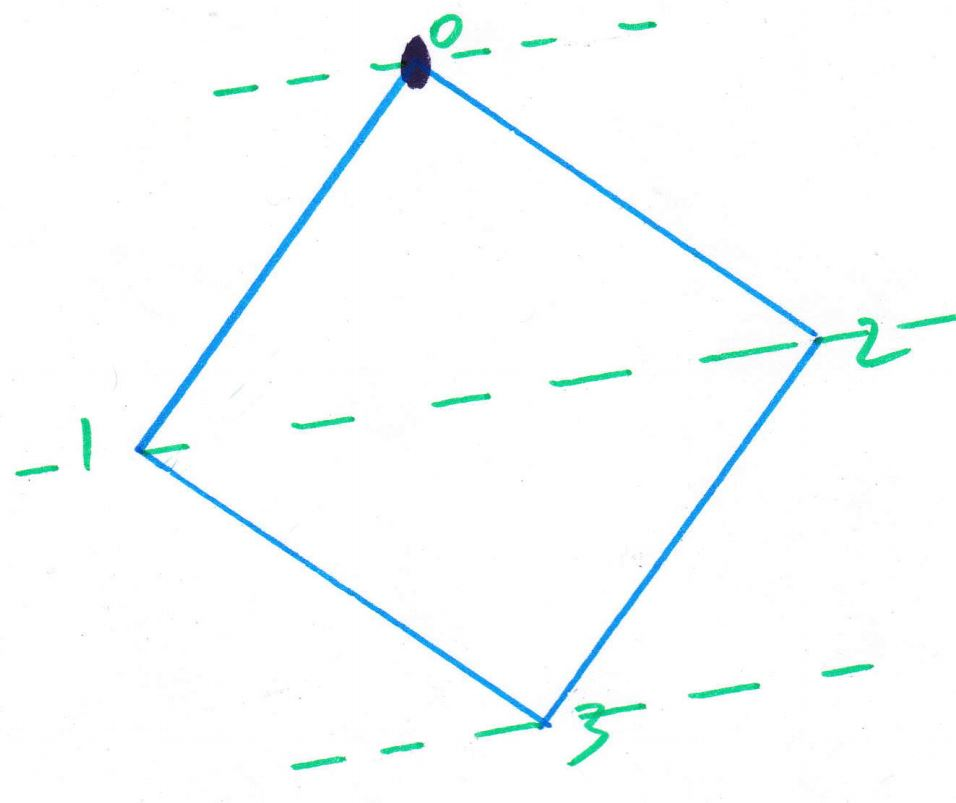
\includegraphics[width=0.5\columnwidth]{figure/2t2.JPG}
\caption{The 2*2 regular network and the root processor is $P_{0}$}
\label{fig:2t2}
\end{figure}

The processor $P_{0}$, $P_{1}$ and $P_{2}$ start to process its respective fraction at the same time.  The processor $P_{3}$ starts to work until the $\alpha_{1}$ and $\alpha_{2}$ are completed transmission.  

According to the divisible load theory\cite{bharadwaj2003divisible}, we obtain the timing diagram \Fig{2t2d}.  

\begin{figure}[!ht]
\centering
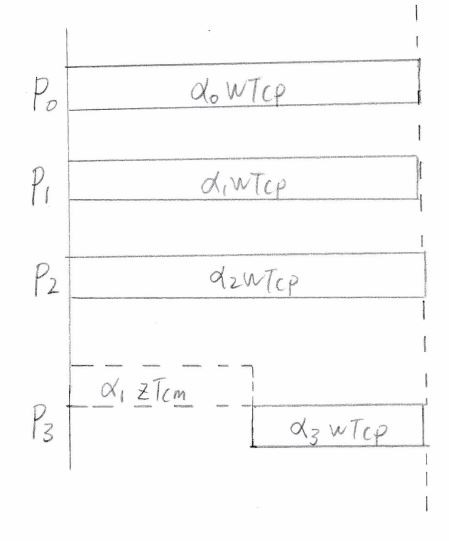
\includegraphics[width=0.5\columnwidth]{figure/2t2d.JPG}
\caption{The timing diagram for 2*2 regular network and the root processor is $P_{0}$}
\label{fig:2t2d}
\end{figure}
Based on the timing diagram, we get a group of equations to deploy the fraction workload:
\\
\begin{empheq}[left=\empheqlbrace]
{align}
\alpha_{0} \omega T_{cp} = T_{f, m}\\
\alpha_{1} \omega T_{cp} = T_{f, m}\\
\alpha_{2} \omega T_{cp} = T_{f, m}\\
\alpha_{1}zT_{cm} + \alpha_{3}\omega T_{cp} = T_{f, m}\\
\alpha_{0} + \alpha_{1} + \alpha_{2} + \alpha_{3} = 1\\
\sigma = \frac{zT_{cm}}{\omega T_{cp}}\\
0 < \sigma < 1 \\
0 < \alpha_{0} \leq  1\\
0 \leq  \alpha_{1},  \alpha_{2},  \alpha_{3}  < 1
\end{empheq}
\\

The group of equations are represented by the matrix form:

\begin{equation}
{
\left[ \begin{array}{ccc}
1 & 2 & 1\\
1 & -1 & 0\\
0 & \sigma-1 & 1
\end{array} 
\right ]} \times \left[ \begin{array}{c}
\alpha_{0} \\
\alpha_{1} \\
\alpha_{3} 
\end{array} 
\right ] = \left[ \begin{array}{c}
1 \\
0 \\
0 
\end{array} 
\right ]
\end{equation}
The matrix is represented as $A \times \alpha = b$.  $A$ is named as \textbf{\textit{flow matrix}}.

Finally, the explicit solution is:
\begin{empheq}[left=\empheqlbrace]
{align}
\sigma = \frac{zT_{cm}}{\omega T_{cp}}\\
\alpha_{0} = \frac{1}{4- \sigma}\\
\alpha_{1} = \frac{1}{4- \sigma}\\
\alpha_{3} = \frac{1 - \sigma}{4- \sigma}
\end{empheq}
\\

The simulation result is illustrated:
\begin{figure}[!ht]
\centering
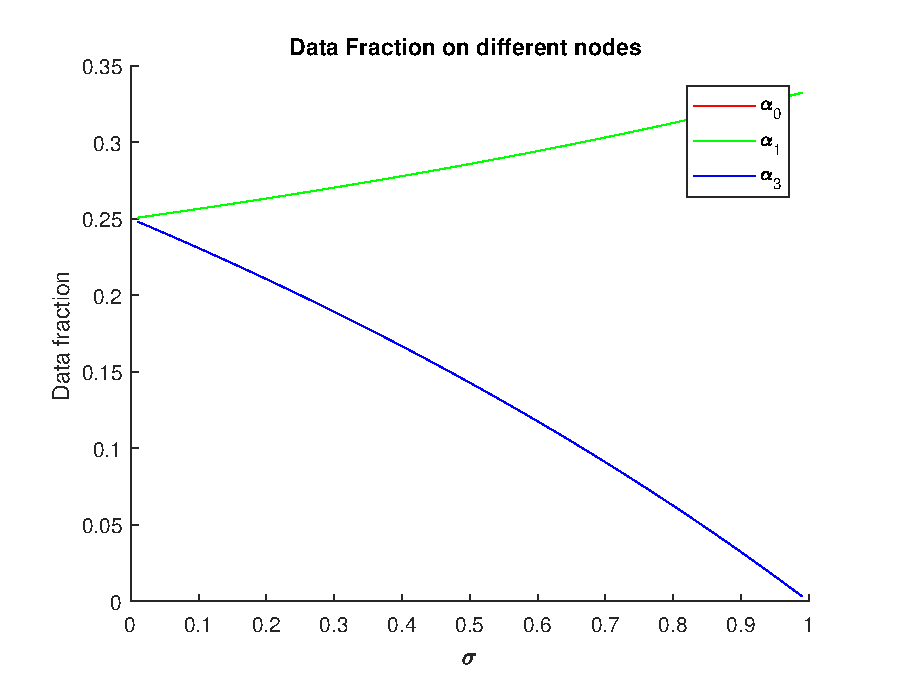
\includegraphics[width=1\columnwidth]{figure/2t2fraction}
\caption{2*2 regular network.  $\alpha_{0}$, $\alpha_{1}$, $\alpha_{2}$, $\alpha_{3}$ value curve}
\label{fig:2t2fraction}
\end{figure}
\newpage 

In \Fig{2t2fraction},  $P_{0}$, $P_{1}$, $P_{2}$ three processors have the same data fraction workload, so the curve of $\alpha_{0}$ and $\alpha_{1}$ coincide.  
The figure says that as $\sigma$ grows,  the value $\alpha_{3}$ drops.  In other words, as the communication capacity decreases, there is less data workload assigned to $P_{3}$.  Further, it means it will be economical to keep the load local on $P_{0}$ nor distribute it to other processors.  

The speedup is:
$$Speedup = \frac{T_{f, 0}}{T_{f, n}}= \frac{\omega T_{cp}}{\alpha_{0}\omega T_{cp}} = \frac{1}{\alpha_{0}} = 4- \sigma$$
\newpage 

\subsubsection{2*3 Regular Network}
In \Fig{2t3} regular network, $L$ happens on processor $P_{0}$.  There are $6$ processors to be processing.  
\begin{figure}[!ht]
\centering
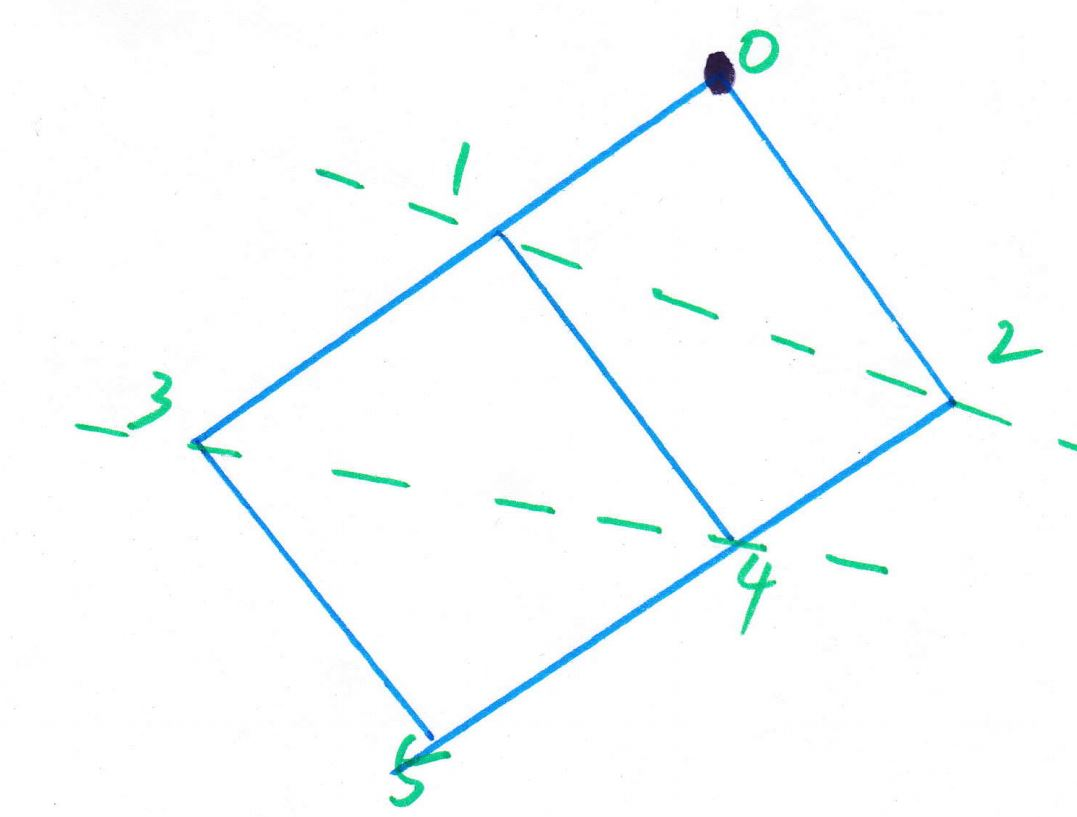
\includegraphics[width=0.5\columnwidth]{figure/2t3.JPG}
\caption{The 2*3 regular network and the data injection happens on corner processor $P_{0}$}
\label{fig:2t3}
\end{figure}

Here $P_{0}$, $P_{1}$ and $P_{2}$ start processing at the same time.  Processor $P_{3}$ and $P_{4}$ start to work when they receive the data from processor $P_{1}$, $P_{2}$.  That is, $P_{3}$ and $P_{4}$ have to wait the fraction of $\alpha_{1}$ and $\alpha_{2}$ are transmitted completely.\\
The last processor $P_{5}$ starts to execute until the work load fraction $\alpha_{0}$, $\alpha_{1}$, $\alpha_{2}$, $\alpha_{3}$, $\alpha_{4}$ are transmitted completed.  According to the divisible load theory\cite{bharadwaj2003divisible}, we obtain the timing diagram \Fig{2t3d}.  

\newpage 
\begin{figure}[!ht]
\centering
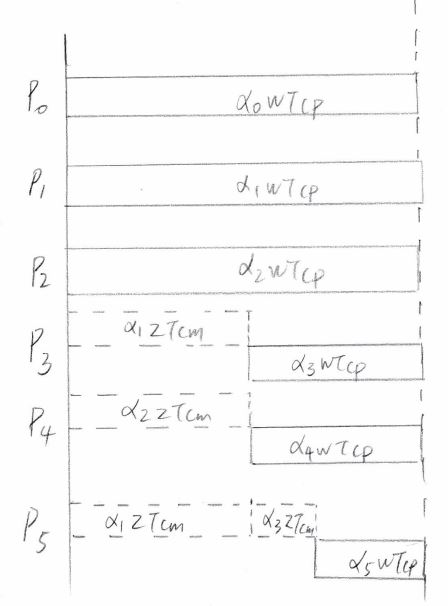
\includegraphics[width=0.5\columnwidth]{figure/2t3d.JPG}
\caption{The timing diagram for a 2*3 regular network and the data injection happens on processor $P_{0}$}
\label{fig:2t3d}
\end{figure}

\newpage

The equations as follows:
\begin{empheq}
[left=\empheqlbrace]
{align}
\alpha_{0} \omega T_{cp} = T_{f, m}\\
\alpha_{1} \omega T_{cp} = T_{f, m}\\
\alpha_{2} \omega T_{cp} = T_{f, m}\\
\alpha_{1}zT_{cm} + \alpha_{3}\omega T_{cp} = T_{f, m}\\
\alpha_{2}zT_{cm} + \alpha_{4}\omega T_{cp} = T_{f, m}\\
(\alpha_{1} + \alpha_{3})zT_{cm} + \alpha_{5}\omega T_{cp} = T_{f, m}\\
\alpha_{0} + \alpha_{1} + \alpha_{2} + \alpha_{3} + \alpha_{4} + \alpha_{5} = 1\\
\sigma = \frac{zT_{cm}}{\omega T_{cp}}\\
0 < \sigma < 1 \\
0 < \alpha_{0} \leq 1\\
0 \leq \alpha_{1},  \alpha_{2},  \alpha_{3} , \alpha_{4} , \alpha_{5} < 1
\end{empheq}
\\

The flow matrix closed-form formula is:
\begin{equation}
{
\left[ \begin{array}{cccc}
1 & 2 & 2 & 1\\
1 & -1 & 0 & 0\\
0 & \sigma-1 & 1 & 0\\
0 & \sigma-1 & \sigma & 1
\end{array} 
\right ]} \times \left[ \begin{array}{c}
\alpha_{0} \\
\alpha_{1} \\
\alpha_{3} \\
\alpha_{5}
\end{array} 
\right ] = \left[ \begin{array}{c}
1 \\
0 \\
0 \\
0
\end{array} 
\right ]
\end{equation}
The explicit solution is:
\begin{empheq}[left=\empheqlbrace]
{align}
\sigma = \frac{zT_{cm}}{\omega T_{cp}}\\
\alpha_{0} = \frac{1}{\sigma^2- 4 \times \sigma + 6}\\
\alpha_{1} = \frac{1}{\sigma^2- 4 \times \sigma + 6}\\
\alpha_{3} = \frac{1 - \sigma}{\sigma^2 - 4 \times \sigma + 6}\\
\alpha_{5} = \frac{\sigma^2 - 2 \times \sigma + 1}{\sigma^2 - 4 \times \sigma + 6}
\end{empheq}
\\
The $\alpha$ calculation result are shown in \Fig{2t3fraction}.  
$P_{0}$,  $P_{1}$ have the same fraction so the curve of $\alpha_{0}$ and $\alpha_{1}$ coincide.  

\begin{figure}[!ht]
\centering
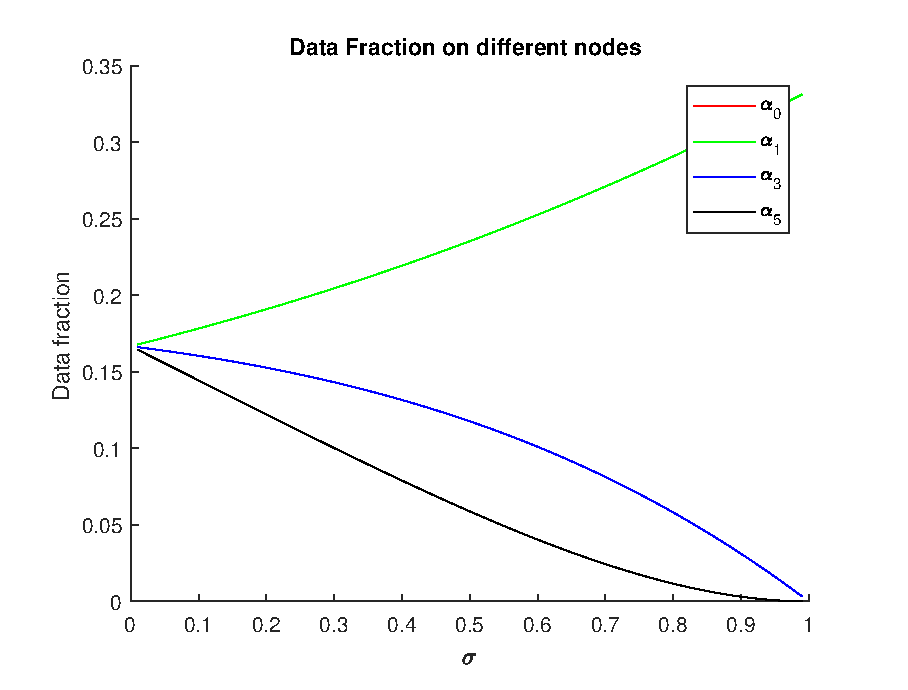
\includegraphics[width=1\columnwidth]{figure/2t3fraction.eps}
\caption{2*2 regular network.  $\alpha_{0}$, $\alpha_{1}$, $\alpha_{3}$, $\alpha_{5}$ data fraction value}
\label{fig:2t3fraction}
\end{figure}

\newpage
\subsubsection*{2*N Regular Network}
The $2*n$ \Fig{2t10} homogeneous regular network address $L_{1}$ at the same time and $L$ happens on $P_{0}$.  

\begin{figure}[!ht]
\centering
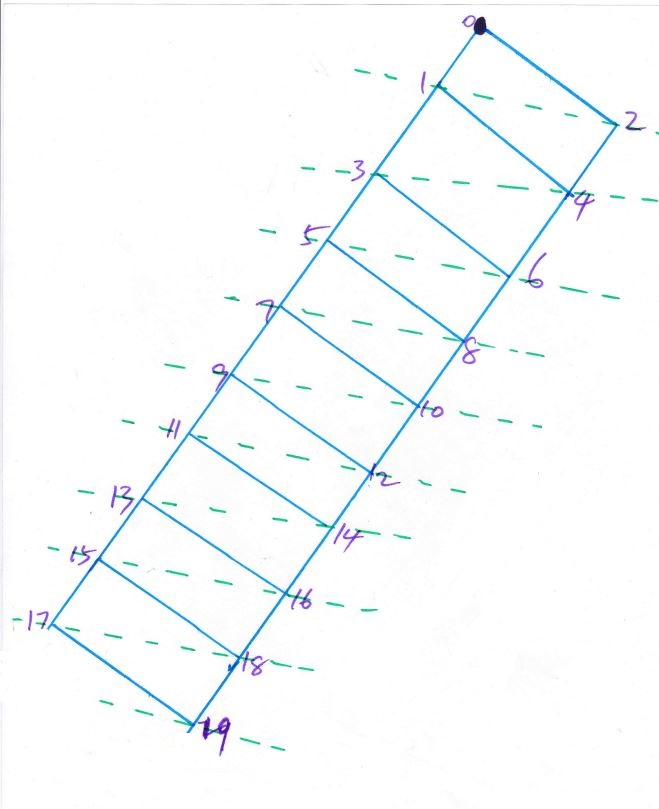
\includegraphics[width=0.6\columnwidth]{figure/2t10.JPG}
\caption{The 2*n (n = 10) regular network and the workload happens on $P_{0}$}
\label{fig:2t10}
\end{figure}
\newpage

Similarly to the analysis of \Fig{2t2d} and \Fig{2t3d},  the timing diagram for \Fig{2t10} is shown in \Fig{2t10d}

\begin{figure}[!ht]
\centering
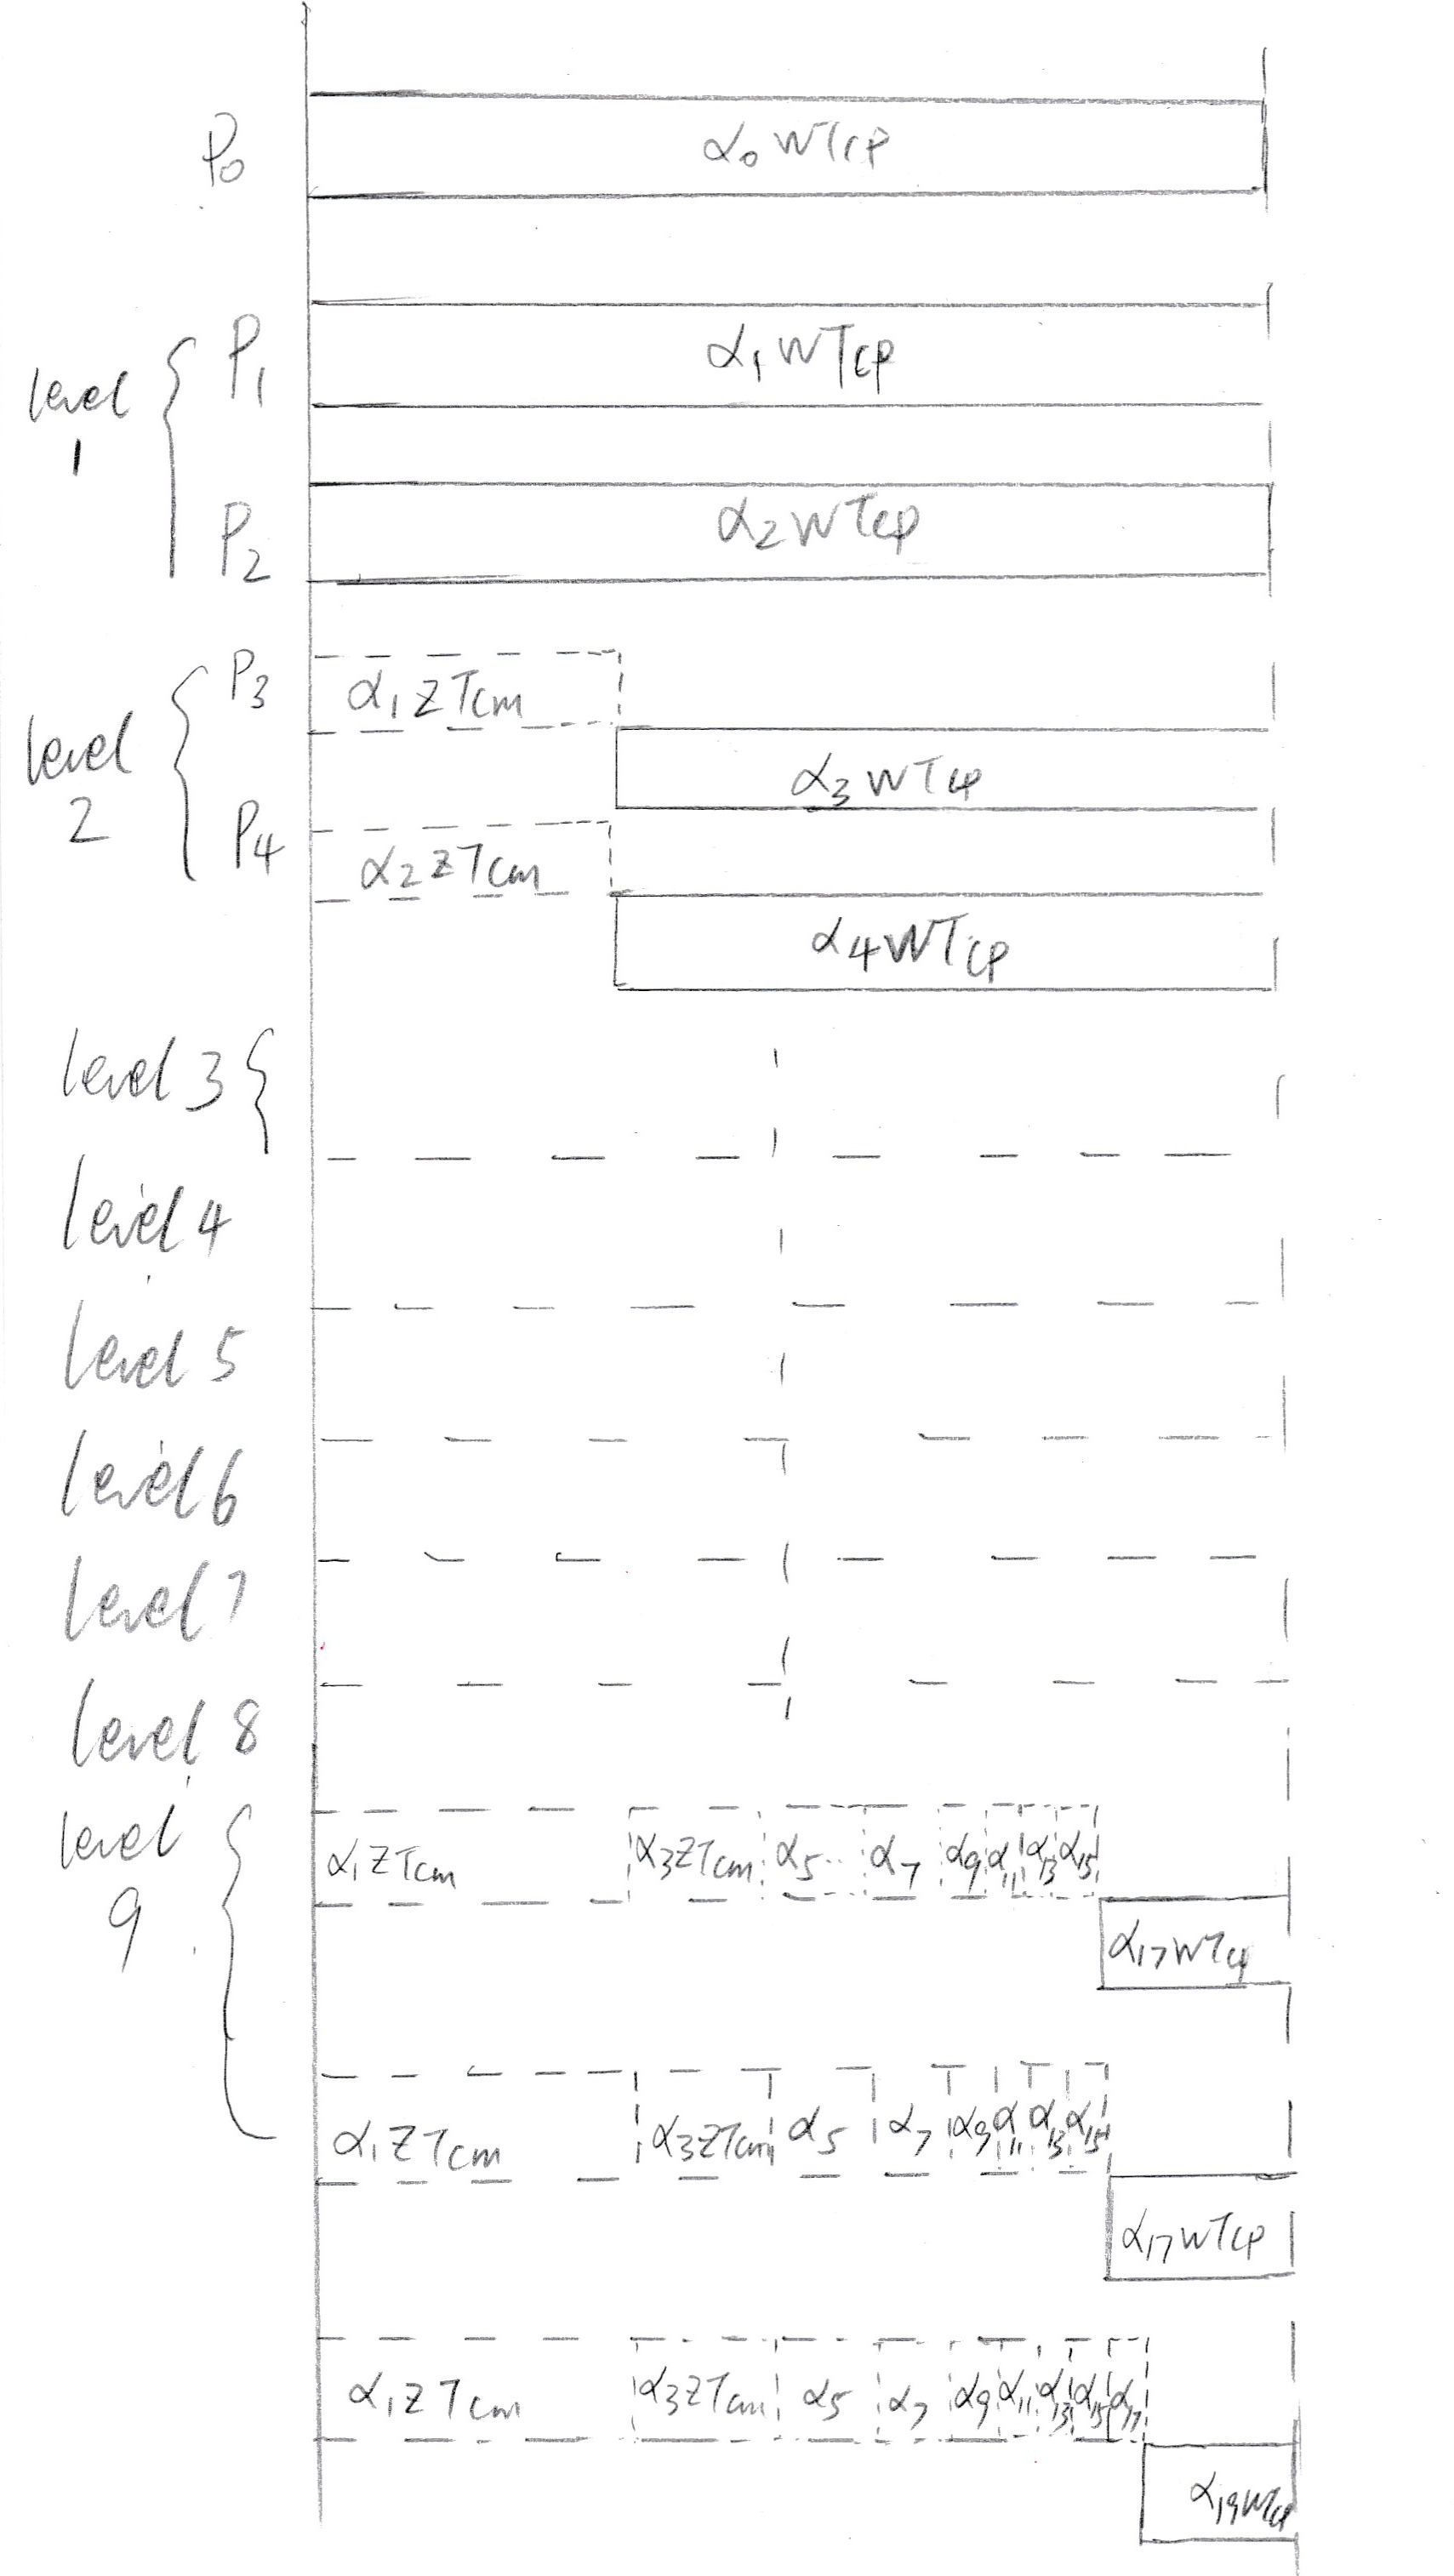
\includegraphics[width=0.7\columnwidth]{figure/2t10d.jpg}
\caption{The timing diagram for 2*10 regular network and the data injection happens on $P_{0}$}
\label{fig:2t10d}
\end{figure}

The equations are presented as:
\begin{empheq}[left=\empheqlbrace]
{align}
\alpha_{0} \omega T_{cp} = T_{f, m}\\
\alpha_{1} \omega T_{cp} = T_{f, m}\\
\alpha_{2} \omega T_{cp} = T_{f, m}\\
\alpha_{1}zT_{cm} + \alpha_{3}\omega T_{cp} = T_{f, m}\\
\alpha_{2}zT_{cm} + \alpha_{4}\omega T_{cp} = T_{f, m}\\
(\alpha_{1} + \alpha_{3})zT_{cm} + \alpha_{5}\omega T_{cp} = T_{f, m}\\
\vdots \\
(\alpha_{1} + \alpha_{3} +\cdots + \alpha_{2 \times n - 1})zT_{cm} +\alpha_{2 \times n - 1} \omega T_{cp} = T_{f, m}\\
\alpha_{0} + \cdots + \alpha_{2 \times n - 1} = 1\\
\sigma = \frac{zT_{cm}}{\omega T_{cp}}\\
0 < \sigma < 1 \\
0 < \alpha_{0} \leq 1\\
0 \leq \quad \alpha_{1} \quad \alpha_{2} \quad  \cdots  \quad \alpha_{2 \times n - 1} < 1
\end{empheq}
\\

The flow matrix closed-form is shown:
\begin{equation}
{
\left[ \begin{array}{ccccccc}
1 & 2 & 2 & \cdots & 2 & 2 & 1\\
1 & -1 & 0 & \cdots& 0 & 0 & 0\\
0 & \sigma-1 & 1 & \cdots & 0 & 0 & 0 \\
0 & \sigma-1 & \sigma & 1 & 0 & \cdots & 0 \\
0 & \sigma-1 & \sigma & \sigma & 1 & 0 & 0 \\
\vdots & \vdots & \vdots  &   \vdots & \ddots & \ddots\\
0 & \sigma-1 & \sigma & \cdots & \sigma & \sigma & 1
\end{array} 
\right ]} \times \left[ \begin{array}{c}
\alpha_{0} \\
\alpha_{1} \\
\alpha_{3} \\
\alpha_{5} \\
\vdots \\
\alpha_{2 \times n - 3}\\
\alpha_{2 \times n - 1}
\end{array} 
\right ] = \left[ \begin{array}{c}
1 \\
0 \\
0 \\
0 \\
\vdots \\
0 \\
0
\end{array} 
\right ]
\end{equation}

According to the \textbf{\textit{Cramer's rule}},the explicit solution for the group of equations is:
\begin{empheq}[left=\empheqlbrace]
{align}
\alpha_{i} = \left |\frac{\det A^{\star}_{i}}{\det A}\right |
\end{empheq}
where $A^{\star}_{i}$ is the matrix formed by replacing the $i$-th column of A by the column vector b.\\
Especially,
\begin{equation}
{
A^{\star}_{0} = \left[ \begin{array}{ccccccc}
1 & 2 & 2 & \cdots & 2 & 2 & 1\\
0 & -1 & 0 & \cdots& 0 & 0 & 0\\
0 & \sigma-1 & 1 & \cdots & 0 & 0 & 0 \\
0 & \sigma-1 & \sigma & 1 & 0 & \cdots & 0 \\
0 & \sigma-1 & \sigma & \sigma & 1 & 0 & 0 \\
\vdots & \vdots & \vdots  &   \vdots & \ddots & \ddots\\
0 & \sigma-1 & \sigma & \cdots & \sigma & \sigma & 1
\end{array} 
\right ]}
\end{equation}

$$\alpha_{0} = \left |\frac{\det A^{\star}_{0}}{\det A} \right |$$
$$\det A^{\star}_{0} = -1$$

Finally, the speedup is:
$$Speedup = \frac{T_{f, 0}}{T_{f, n}}= \frac{\omega T_{cp}}{\alpha_{0}\omega T_{cp}} = \frac{1}{\alpha_{0}} =  \left|-\det A\right|$$.

Further, we prove the matrix $\det A \neq 0$. 
\renewcommand{\qedsymbol}{$\blacksquare$}

\begin{equation}
{
C = \left[ \begin{array}{cccccc}
-1 & 0 & \cdots& 0 & 0 & 0\\
\sigma-1 & 1 & \cdots & 0 & 0 & 0 \\
\sigma-1 & \sigma & 1 & 0 & \cdots & 0 \\
\sigma-1 & \sigma & \sigma & 1 & 0 & 0 \\
\vdots & \vdots & \vdots  &   \vdots & \ddots & \ddots\\
\sigma-1 & \sigma & \cdots & \sigma & \sigma & 1
\end{array} 
\right ]
}
\end{equation}

$C$ is a lower triangular matrix and the diagonal elements are not $0$.  So $C$ is non-degenerate, that is, the matrix is column linear independence.

After a series of column reduction and row reduction actions, we get
\begin{equation*}
     {A = \left[ \begin{array}{ccccccc}
1 & 2 & 2 & \cdots & 2 & 2 & 1\\
1 & -1 & 0 & \cdots& 0 & 0 & 0\\
0 & \sigma-1 & 1 & \cdots & 0 & 0 & 0 \\
0 & \sigma-1 & \sigma & 1 & 0 & \cdots & 0 \\
0 & \sigma-1 & \sigma & \sigma & 1 & 0 & 0 \\
\vdots & \vdots & \vdots  &   \vdots & \ddots & \ddots\\
0 & \sigma-1 & \sigma & \cdots & \sigma & \sigma & 1
\end{array} 
\right ]
\xrightarrow[\text{Reduction}]{\text{Column}}\\
\left[ \begin{array}{ccccccc}
1 & 0 & 0 & \cdots & 0 & 0 & 0\\
1 & -3 & -2 & \cdots& -2 & -2 & -1\\
0 & \sigma-1 & 1 & \cdots & 0 & 0 & 0 \\
0 & \sigma-1 & \sigma & 1 & 0 & \cdots & 0 \\
0 & \sigma-1 & \sigma & \sigma & 1 & 0 & 0 \\
\vdots & \vdots & \vdots  &   \vdots & \ddots & \ddots\\
0 & \sigma-1 & \sigma & \cdots & \sigma & \sigma & 1
\end{array} 
\right ]
}
\end{equation*}

\begin{equation*}
{\xrightarrow[\text{Reduction}]{\text{Row}}\\
\left[ \begin{array}{ccccccc}
1 & 0 & 0 & \cdots & 0 & 0 & 0\\
0 & -3 & -2 & \cdots& -2 & -2 & -1\\
0 & \sigma-1 & 1 & \cdots & 0 & 0 & 0 \\
0 & \sigma-1 & \sigma & 1 & 0 & \cdots & 0 \\
0 & \sigma-1 & \sigma & \sigma & 1 & 0 & 0 \\
\vdots & \vdots & \vdots  &   \vdots & \ddots & \ddots\\
0 & \sigma-1 & \sigma & \cdots & \sigma & \sigma & 1
\end{array} 
\right ]
}
\end{equation*}
Considering the matrix $\hat{C}$
\begin{equation}
{
\hat{C} = \left[ \begin{array}{cccccc}
-3 & -2 & \cdots& -2 & -2 & -1\\
\sigma-1 & 1 & \cdots & 0 & 0 & 0 \\
\sigma-1 & \sigma & 1 & 0 & \cdots & 0 \\
\sigma-1 & \sigma & \sigma & 1 & 0 & 0 \\
\vdots & \vdots & \vdots  &   \vdots & \ddots & \ddots\\
\sigma-1 & \sigma & \cdots & \sigma & \sigma & 1
\end{array} 
\right ]
}
\end{equation}
, which is still column linear independence.  Considering $0 < \sigma < 1$, the flow matrix is full rank. So $\det A \neq 0$.

After three user cases' investigation, we find a crucial rule:
\textbf{$$\forall D_{i} = D_{j}, \quad then \quad \alpha_{i} = \alpha_{j},  \quad  0 \leq i,  j \leq m*n-1$$}

\newpage

\subsubsection*{m*n Regular Network}
Considering a general $m*n$ regular network,  such as \Fig{3t8} \Fig{5t5}.  

\begin{figure}[!ht]
\centering
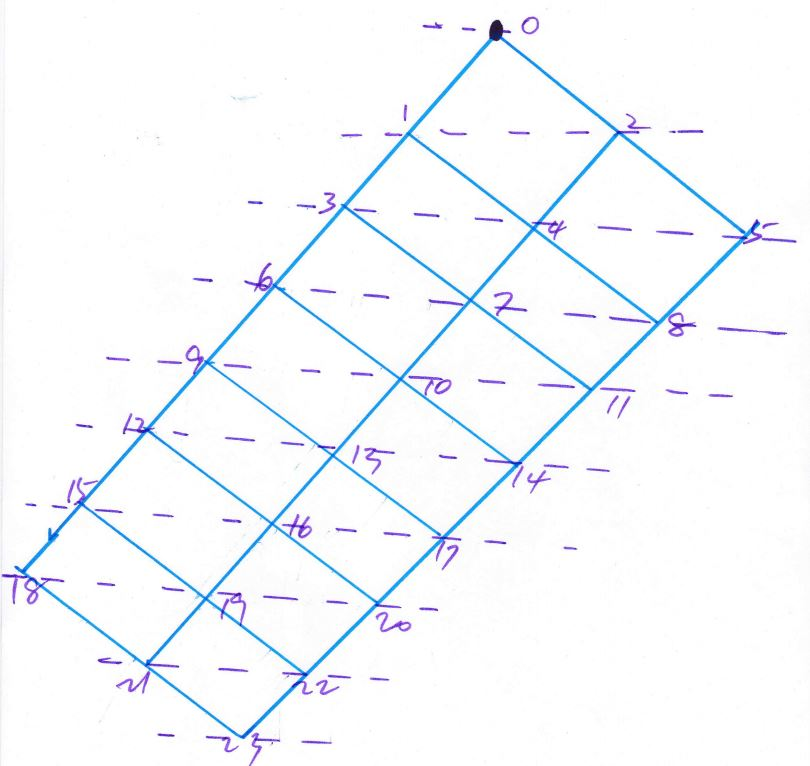
\includegraphics[width=0.55\columnwidth]{figure/3t8.JPG}
\caption{3*8 regular network.  The data injection position is $P_{0}$}
\label{fig:3t8}
\end{figure}

\begin{figure}[!ht]
\centering
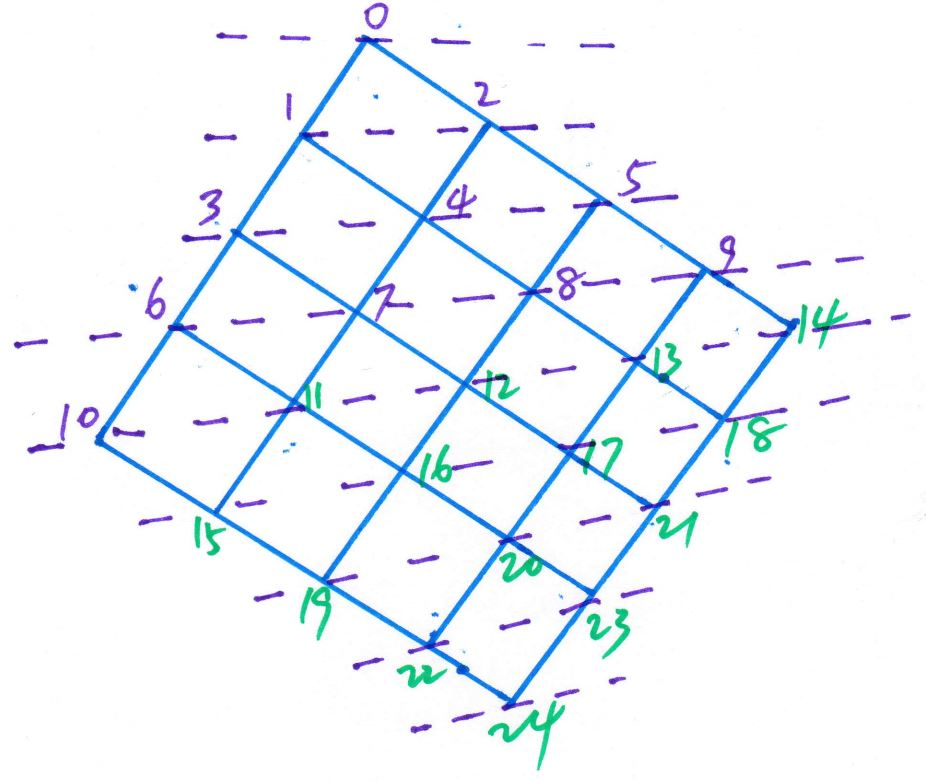
\includegraphics[width=0.55\columnwidth]{figure/5t5.JPG}
\caption{5*5 regular network.  The data injection position is $P_{0}$}
\label{fig:5t5}
\end{figure}

Utilizing the rule, we obtain the closed-form flow matrix equations for \Fig{3t8}:
\begin{equation}
{
\left[ \begin{array}{cccccccccc}
1 & 2 & 3 & 3 & 3 & 3 & 3 & 3 & 2 & 1\\
1 & -1 & 0 & 0 & 0 & 0 & 0 & 0 & 0 & 0\\
0 & \sigma-1 & 1 & 0 & 0 & 0 & 0 & 0 & 0 & 0 \\
0 & \sigma-1 & \sigma & 1 & 0 & 0 & 0 & 0 & 0 & 0 \\
0 & \sigma-1 & \sigma & \sigma & 1 & 0 & 0 & 0 & 0 & 0\\
0 & \sigma-1 & \sigma & \sigma & \sigma & 1 & 0 & 0 & 0 & 0\\
0 & \sigma-1 & \sigma & \sigma & \sigma & \sigma & 1 & 0 & 0 & 0\\
0 & \sigma-1 & \sigma & \sigma & \sigma & \sigma & \sigma & 1 & 0 & 0\\
0 & \sigma-1 & \sigma & \sigma & \sigma & \sigma & \sigma & \sigma & 1 & 0\\
0 & \sigma-1 & \sigma & \sigma & \sigma & \sigma & \sigma & \sigma & \sigma & 1 \\
\end{array} 
\right ]} \times \left[ \begin{array}{c}
\alpha_{0} \\
\alpha_{1} \\
\alpha_{3} \\
\alpha_{6} \\
\alpha_{9} \\
\alpha_{12}\\
\alpha_{15}\\
\alpha_{18}\\
\alpha_{21}\\
\alpha_{23}
\end{array} 
\right ] = \left[ \begin{array}{c}
1 \\
0 \\
0 \\
0 \\
0 \\
0 \\
0 \\
0 \\
\vdots \\
0
\end{array} 
\right ]
\end{equation}

Also, the flow matrix equations for \Fig{5t5}:
\begin{equation}
{
\left[ \begin{array}{ccccccccc}
1 & 2 & 3 & 4 & 5 & 4 & 3 & 2 & 1\\
1 & -1 & 0 & 0 & 0 & 0 & 0 & 0& 0\\
0 & \sigma-1 & 1 & 0 & 0 & 0 &0 & 0 & 0 \\
0 & \sigma-1 & \sigma & 1 & 0 & 0 & 0 & 0 & 0 \\
0 & \sigma-1 & \sigma & \sigma & 1 & 0 & 0 & 0 & 0\\
0 & \sigma-1 & \sigma & \sigma & \sigma & 1 & 0& 0 & 0\\
0 & \sigma-1 & \sigma & \sigma & \sigma & \sigma & 1 & 0 & 0\\
0 & \sigma-1 & \sigma & \sigma & \sigma & \sigma & \sigma & 1 & 0\\
0 & \sigma-1 & \sigma & \sigma & \sigma & \sigma & \sigma & \sigma & 1\\
\end{array} 
\right ]} \times \left[ \begin{array}{c}
\alpha_{0} \\
\alpha_{1} \\
\alpha_{3} \\
\alpha_{6} \\
\alpha_{10} \\
\alpha_{15}\\
\alpha_{19}\\
\alpha_{22}\\
\alpha_{24}
\end{array} 
\right ] = \left[ \begin{array}{c}
1 \\
0 \\
0 \\
0 \\
0 \\
0 \\
0 \\
\vdots \\
0
\end{array} 
\right ]
\end{equation}

We use the similar method to prove $\det A \neq 0$, so the speedup is:
$$Speedup = \frac{T_{f, 0}}{T_{f, n}}= \frac{\omega T_{cp}}{\alpha_{0}\omega T_{cp}} = \frac{1}{\alpha_{0}} = \left |-\det A \right |$$.

\subsection{Data Injection On The Boundary Processor}
After the corner scenario,  we extend the rule to boundary processor condition.  \\
If the single data injection roots on the boundary processor, for example \Fig{3t3b}.  
\begin{figure}[!ht]
\centering
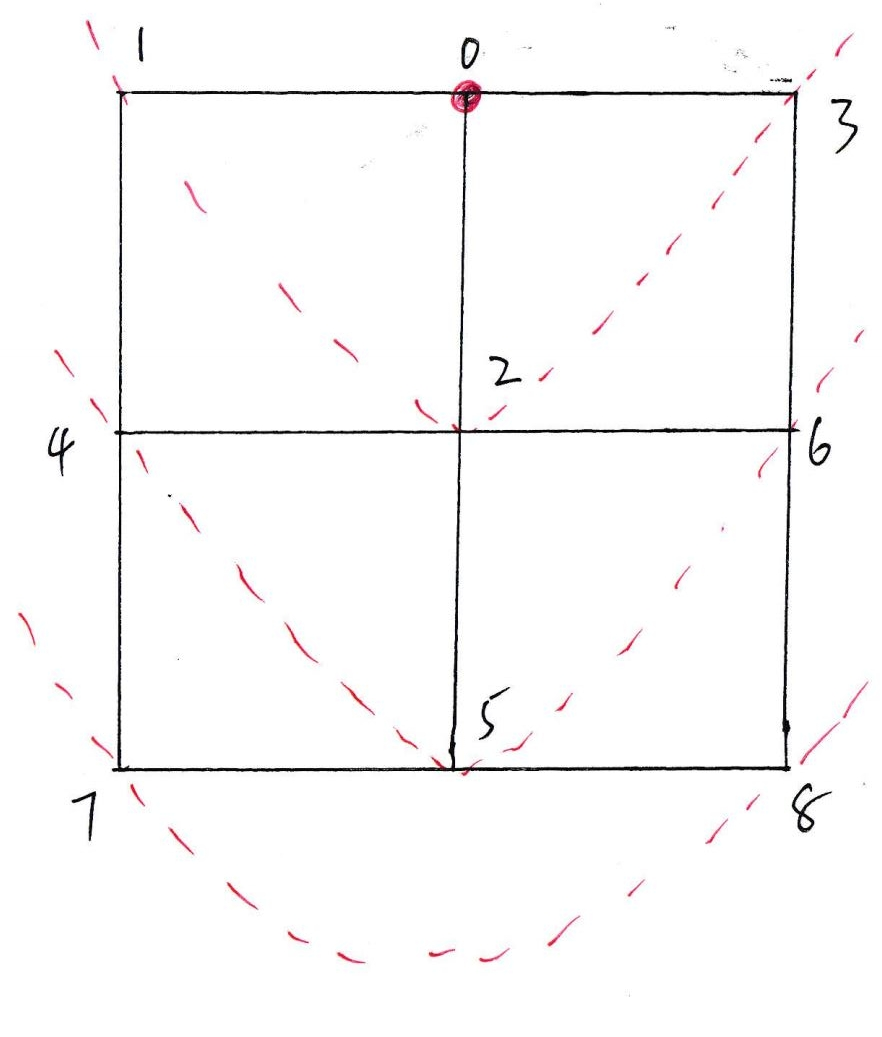
\includegraphics[width=0.5\columnwidth]{figure/3t3b.JPG}
\caption{The 3*3 regular network and the root processor is $P_{0}$}
\label{fig:3t3b}
\end{figure}
\newpage 

The timing diagram is \Fig{3t3bd}:
\begin{figure}[!ht]
\centering
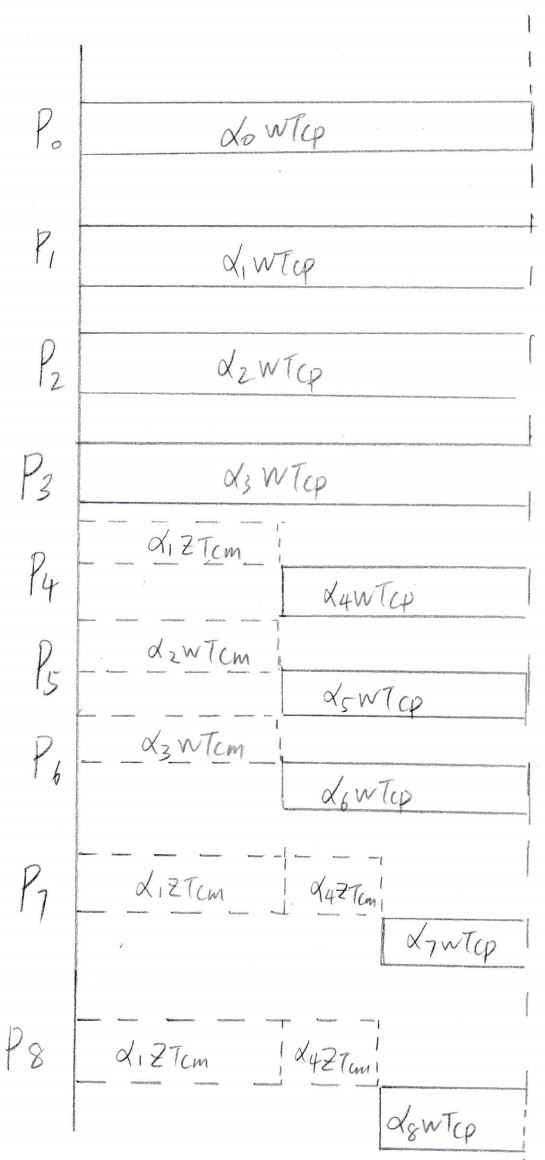
\includegraphics[width=0.5\columnwidth]{figure/3t3bd.JPG}
\caption{The timing diagram for 3*3 regular network and the data injection occurs on $P_{0}$}
\label{fig:3t3bd}
\end{figure}
\newpage 

The equations are:
\begin{empheq}[left=\empheqlbrace]
{align}
\alpha_{0} \omega T_{cp} = T_{f, m}\\
\alpha_{1} \omega T_{cp} = T_{f, m}\\
\alpha_{2} \omega T_{cp} = T_{f, m}\\
\alpha_{3} \omega T_{cp} = T_{f, m}\\
\alpha_{1}zT_{cm} + \alpha_{4}\omega T_{cp} = T_{f, m}\\
\alpha_{2}zT_{cm} + \alpha_{5}\omega T_{cp} = T_{f, m}\\
\alpha_{3}zT_{cm} + \alpha_{6}\omega T_{cp} = T_{f, m}\\
(\alpha_{1} + \alpha_{4})zT_{cm} + \alpha_{7}\omega T_{cp} = T_{f, m}\\
(\alpha_{2} + \alpha_{5})zT_{cm} + \alpha_{8}\omega T_{cp} = T_{f, m}\\
\alpha_{0} + \cdots + \alpha_{8} = 1\\
\sigma = \frac{zT_{cm}}{\omega T_{cp}}\\
0 < \sigma < 1 \\
0 < \alpha_{0} \leq 1\\
0 \leq  \quad \alpha_{1} \quad \alpha_{2} \quad  \cdots  \quad \alpha_{8} < 1\\
\end{empheq}
\newpage

And the flow matrix form is :
\begin{equation}
{
\left[ \begin{array}{cccc}
1 & 3 & 3 & 2\\
1 & -1 & 0 & 0\\
0 & \sigma-1 & 1 & 0\\
0 & \sigma-1 & \sigma & 1
\end{array} 
\right ]} \times \left[ \begin{array}{c}
\alpha_{0} \\
\alpha_{1} \\
\alpha_{4} \\
\alpha_{7}
\end{array} 
\right ] = \left[ \begin{array}{c}
1 \\
0 \\
0 \\
0
\end{array} 
\right ]
\end{equation}
The explicit solution is:
\begin{empheq}[left=\empheqlbrace]
{align}
\alpha_{0} = \frac{1}{9 - 7\times \sigma + 2 \times \sigma^{2}}\\
\alpha_{1} = \frac{1}{9 - 7\times \sigma + 2 \times \sigma^{2}}\\
\alpha_{4} = \frac{1-\sigma}{9 - 7\times \sigma + 2 \times \sigma^{2}}\\
\alpha_{7} = \frac{(1-\sigma)^{2}}{9 - 7\times \sigma + 2 \times \sigma^{2}}\\
\end{empheq}

The simulation result is shown:
\begin{figure}[!ht]
\centering
\includegraphics[width=1\columnwidth]{figure/3t3bfraction.eps}
\caption{The data fraction simulation result of 3*3 regular network and the data injection happens on the boundary $P_{0}$}
\label{fig:3t3bfraction}
\end{figure}
$P_{0}$ and $P_{1}$ have the same $\alpha$, so the curve of $\alpha_{0}$ and $\alpha_{1}$ coincide.  
\newpage 
\subsection{Data Injection On The Inner Grid Processor}

\Fig{3t3i} shows that $L$ loads on the inner grid processor $P_{0}$, 
\begin{figure}[!ht]
\centering
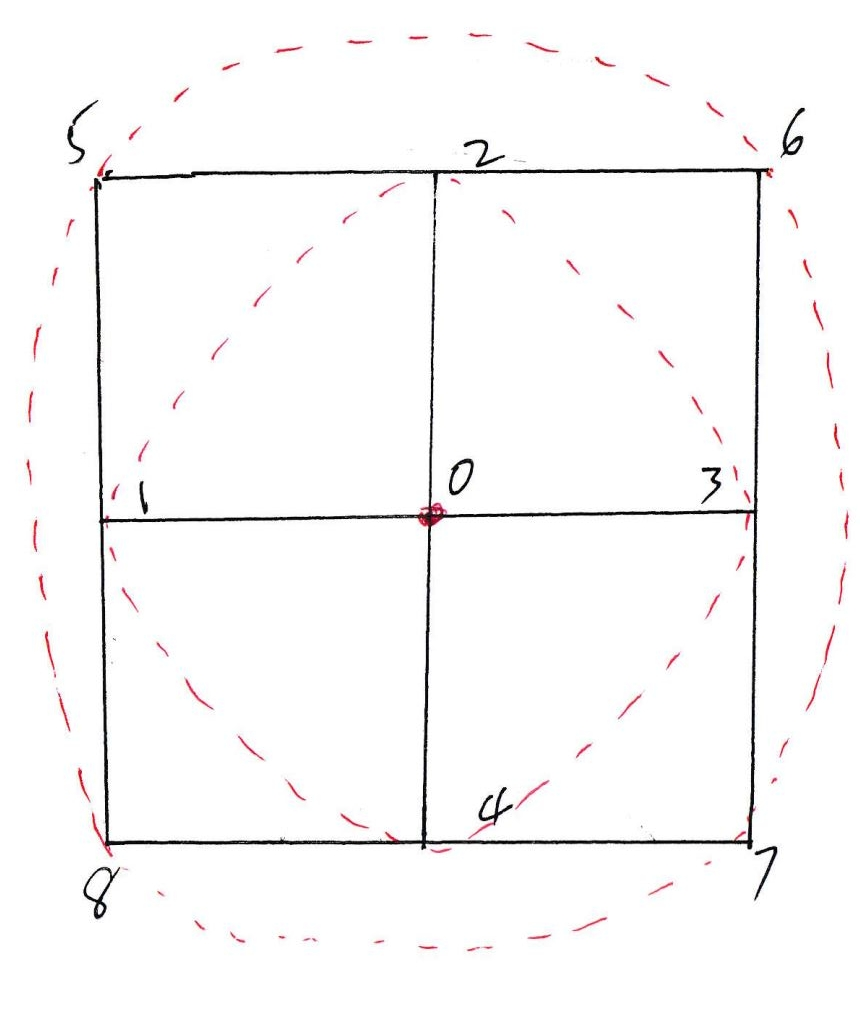
\includegraphics[width=0.5\columnwidth]{figure/3t3i.JPG}
\caption{3*3 regular network.  The data injection position is inner grid point $P_{0}$}
\label{fig:3t3i}
\end{figure}
\newpage

The timing diagram for this user case is illustrated as \Fig{3t3id}:
\begin{figure}[!ht]
\centering
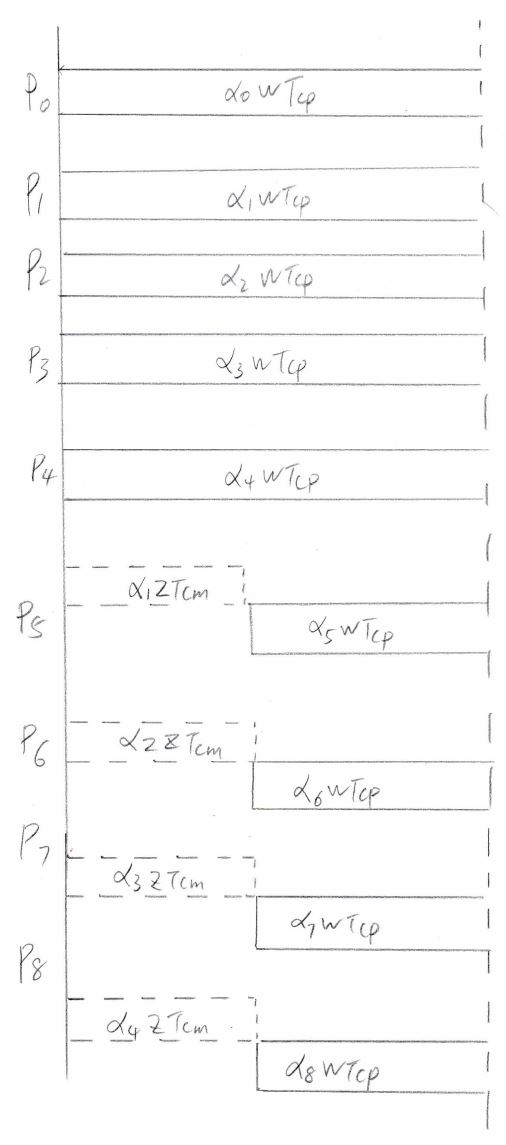
\includegraphics[width=0.55\columnwidth]{figure/3t3id.JPG}
\caption{The timing diagram for 3*3 regular network and the data injection is inner grid $P_{0}$}
\label{fig:3t3id}
\end{figure}
\newpage 

The group of equations are:
\begin{empheq}[left=\empheqlbrace]
{align}
\alpha_{0} \omega T_{cp} = T_{f, m}\\
\alpha_{1} \omega T_{cp} = T_{f, m}\\
\alpha_{2} \omega T_{cp} = T_{f, m}\\
\alpha_{3} \omega T_{cp} = T_{f, m}\\
\alpha_{4} \omega T_{cp} = T_{f, m}\\
\alpha_{1}zT_{cm} + \alpha_{5}\omega T_{cp} = T_{f, m}\\
\alpha_{1}zT_{cm} + \alpha_{6}\omega T_{cp} = T_{f, m}\\
\alpha_{1}zT_{cm} + \alpha_{7}\omega T_{cp} = T_{f, m}\\
\alpha_{1}zT_{cm} + \alpha_{8}\omega T_{cp} = T_{f, m}\\
\sigma = \frac{zT_{cm}}{\omega T_{cp}}\\
0 < \sigma < 1 \\
0 < \alpha_{0} \leq 1\\
0 \leq \quad \alpha_{1} \quad \alpha_{2} \quad  \cdots  \quad \alpha_{8} < 1
\end{empheq}
\\

The flow matrix form is :
\begin{equation}
{
\left[ \begin{array}{ccc}
1 & 4 & 4 \\
1 & -1 & 0\\
0 & \sigma-1 & 1\\
\end{array} 
\right ]} \times \left[ \begin{array}{c}
\alpha_{0} \\
\alpha_{1} \\
\alpha_{5} \\
\end{array} 
\right ] = \left[ \begin{array}{c}
1 \\
0 \\
0 
\end{array} 
\right ]
\end{equation}
\newpage 

The simulation result is \Fig{3t3ifraction}:
$P_{0}$ and $P_{1}$ have the same $\alpha$ value, so the curve of $\alpha_{0}$ and $\alpha_{1}$ coincide.  

\begin{figure}[!ht]
\centering
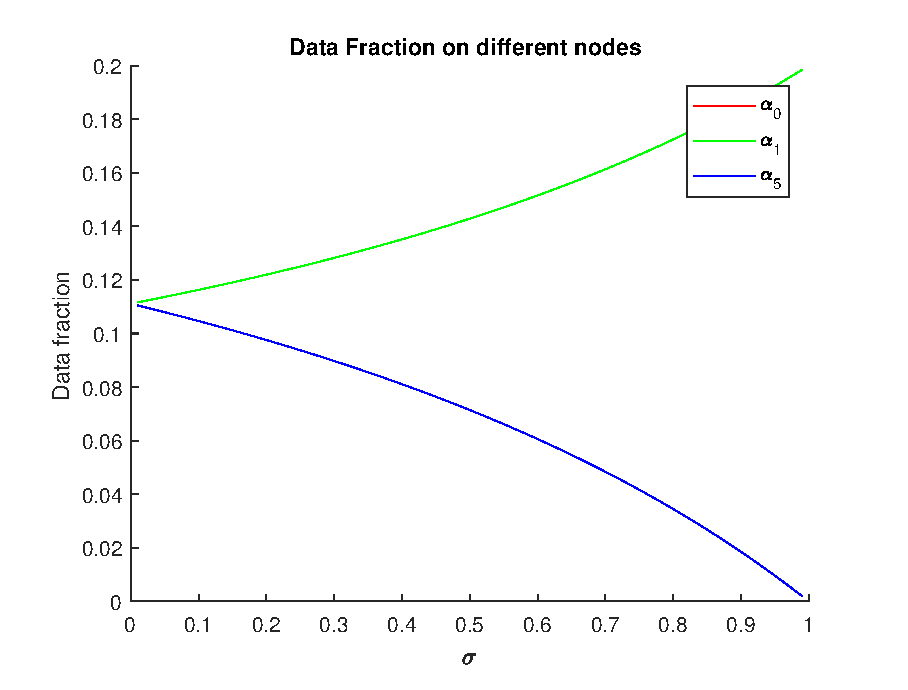
\includegraphics[width=1\columnwidth]{figure/3t3ifraction.eps}
\caption{3*3 regular network.  The data injection position is inner grid point $P_{0}$}
\label{fig:3t3ifraction}
\end{figure}